\documentclass[12pt]{article}

\usepackage{fullpage}
\usepackage{multicol,multirow}
\usepackage{tabularx}
\usepackage{ulem}
\usepackage[utf8]{inputenc}
\usepackage[russian]{babel}
\usepackage{amsmath}
\usepackage{amssymb}
\usepackage{graphicx}
\graphicspath{./}
\usepackage{color}
\usepackage{titlesec}

\titleformat{\section}
  {\normalfont\Large\bfseries}{\thesection.}{0.3em}{}

\titleformat{\subsection}
  {\normalfont\large\bfseries}{\thesubsection.}{0.3em}{}

\titlespacing{\section}{0pt}{*2}{*2}
\titlespacing{\subsection}{0pt}{*1}{*1}
\titlespacing{\subsubsection}{0pt}{*0}{*0}
\usepackage{listings}
\lstloadlanguages{Lisp}
\lstset{extendedchars=false,
	breaklines=true,
	breakatwhitespace=true,
	keepspaces = true,
	tabsize=2
}
\begin{document}


\section*{Отчет по лабораторной работе №\,5
по курсу \guillemotleft  Функциональное программирование\guillemotright}
\begin{flushright}
Студент группы 8О-308 МАИ \textit{Балес Александр}, \textnumero 3 по списку \\
\makebox[7cm]{Контакты: {\tt aleks\_bales@mail.ru} \hfill} \\
\makebox[7cm]{Работа выполнена: 22.05.2016 \hfill} \\
\ \\
Преподаватель: Иванов Дмитрий Анатольевич, доц. каф. 806 \\
\makebox[7cm]{Отчет сдан: \hfill} \\
\makebox[7cm]{Итоговая оценка: \hfill} \\
\makebox[7cm]{Подпись преподавателя: \hfill} \\

\end{flushright}

\section{Тема работы}
Обобщённые функции, методы и классы объектов.

\section{Цель работы}
Научиться определять простейшие классы, порождать экземпляры классов, считывать и изменять значения слотов, научиться определять обобщённые функции и методы.

\section{Задание(вариант 5.25)}
Дан экземпляр класса {\color{blue}\tt{triangle}}, причем все вершины треугольника могут быть заданы как декартовыми координатами (экземплярами класса {\color{blue}\tt{cart}}), так и полярными (экземплярами класса {\color{blue}\tt{polar}}).

Задание: Определить обычную функцию медиана, возвращающую объект-отрезок (экземпляр класса {\color{blue}\tt{line}}), являющийся медианой первого угла \tt{vertex1}. Концы результирующего отрезка могут быть получены либо в декартовых, либо в полярных координатах.
\begin{verbatim}
(setq tri (make-instance 'triangle
           :1 (make-instance 'cart-или-polar ...)
           :2 (make-instance 'cart-или-polar ...)
           :3 (make-instance 'cart-или-polar ...)))
(медиана tri) => [ОТРЕЗОК ...]
\end{verbatim}

\section{Оборудование студента}
Процессор Intel Core i5-3210 4\,@\,2.5GHz, память: 8192Mb, разрядность системы: 64.

\section{Программное обеспечение}
ОС Ubuntu 14.04, среда GNU Common Lisp 2.6.10

\section{Идея, метод, алгоритм}
Все классы и обобщенные ф-ии были взяты и модернизированы с лекций, а ф-ия {\color{red}\tt{median}} выполняет примерно следующие действия: нам необходимо получить отрезок, соединяющий точку \tt{vertex1} треугольника с точкой лежащей на середине стороны, противоположной \tt{vertex1}. Иными словами, медиана опущенная из вершины \tt{vertex1}. Чтобы найти середины отрезка противоположной стороны, необходимо сложить координаты вершин \tt{vertex2} и \tt{vertex3}, и поделить координы на два. В случае же полярной системы координат, нам достаточно уметь приводить полярные координаты к декартовым.
%\section{Сценарий выполнения работы}
\section{Распечатка программы и её результаты}
\lstinputlisting{./lr5.lsp}
\subsection{Результаты}
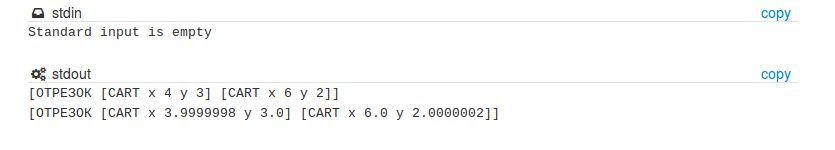
\includegraphics[scale=0.7]{lr5Screen}

%\subsection{Результаты работы}
%\lstinputlisting{./log2.lsp}

%\section{Дневник отладки}
%\begin{tabular}{|c|p{5cm}|p{5cm}|p{3cm}|}
%\hline
%Дата & Событие & Действие по исправлению & Примечание \\
%\hline
%\hline 
%\end{tabular}

\section{Замечания, выводы}
Я приобрел навыки работы с простейшими классами, научился порождать экземпляры классов, считывать и изменять значения слотов, а также определять обобщённые функции и методы.
\end{document}
